\documentclass[12pt,twoside]{article} 

\usepackage{tikz}
\usepackage{textcomp}
\usepackage[siunitx]{circuitikz}
\usepackage{siunitx}
\usepackage{systeme}
\usepackage{graphicx}
\usepackage{listings}
\usepackage{float}
\renewcommand{\contentsname}{Cuprins}


\begin{document}

\title{\begin{huge}
Tema 1
\end{huge}\\
{\small - Bazele electrotehnicii - }}
\author{{\em Adam Robert-Mihai} \\
robert\_mihai.adam@stud.acs.upb.ro\\
Grupa 312AC\\ 
Facultatea de Automatică și Calculatoare\\
Universitatea Politehnică din București \\}
\date{\today} 
\maketitle

\newpage

\tableofcontents
\newpage

\section{Generarea circuitului}

Circuitul este:
\begin{center}
\begin{circuitikz}[american]
\draw (0, 2) to[R, l_=$R_3$,a^=8<\ohm>] (0, 4);
\draw[blue] (2.5, 4) to[R, l_=$R_1$,a^=10<\ohm>, color=blue] (6.5, 4);
\draw[blue] (6.5, 4) to[R, l_=$R_4$,a^=6<\ohm>, color=blue] (6.5, 0);
\draw[blue] (2.5, 4) to[R, l_=$R_2$,a^=8<\ohm>, color=blue] (2.5, 2.5);
\draw (2.5, 0) to[R, l_=$R_5$,a^=12<\ohm>] (4.5, 0);
\draw[blue] (2.5, 2.5) to[V<=15V, color=blue] (2.5, 0);
\draw (6.5,6.5) to[V<=30V] (2.5,6.5);
\draw (0,2) to[V>=15V] (0,0);
\draw (2.5,6.5) to[short] (2.5,4)node[label={[yshift=0.2cm, xshift=-7]right:$(1)$}]{};
\draw (6.5, 6.5) to[short] (6.5,4)node[label={[yshift=0.2cm, xshift=-7]right:$(2)$}]{};
\draw (0,0) to[short] (2.5,0)node[label={[font=\footnotesize]below:$(4)$}] {};
\draw (0,4) to[short] (2.5,4);
\draw (6.5, 4) to[short] (9,4);
\draw (9, 0) to[short] (6.5,0)node[label={[font=\footnotesize]below:$(3)$}] {};
\draw (9, 4) to[I>=4A] (9, 0) node[label={[font=\footnotesize]}]{};
\draw (6.5, 0) to [I>=10A] (4.5,0) node[label={[font=\footnotesize]}]{};
\end{circuitikz}
\end{center}


Graful de intensități:
\begin{center}
\begin{circuitikz}[american]
\draw (0, 0) to[short, i>=5A] (0, 4);
\draw (2.5, 4) to[short, i<=3A]  (6.5, 4);
\draw (6.5, 4) to[short, i>=6A](6.5, 0);
\draw (2.5, 4) to[short, i<=5A] (2.5, 0);
\draw (6.5,6.5) to[short] (2.5,6.5);
\draw (2.5,6.5) to[short] (2.5,4)node[label={[yshift=0.2cm, xshift=-7]right:$(1)$}]{};
\draw (6.5, 6.5) to[short, i>=13A] (6.5,4)node[label={[yshift=0.2cm, xshift=-7]right:$(2)$}]{};
\draw (0,0) to[short] (2.5,0)node[label={[font=\footnotesize]below:$(4)$}] {};
\draw (0,4) to[short] (2.5,4);
\draw (6.5, 4) to[short] (9,4);
\draw (9, 0) to[short] (6.5,0)node[label={[font=\footnotesize]below:$(3)$}] {};
\draw (9, 4) to[short, i>=4A] (9, 0) ;
\draw (6.5, 0) to[short, i>=10A] (2.5,0);
\end{circuitikz}
\end{center}


\newpage
Graful de tensiuni:
\begin{center}
\begin{circuitikz}[american]
\draw (0, 0) to[short, i>=25] (0, 4);
\draw (2.5, 4) to[short, i<=30]  (6.5, 4);
\draw (6.5, 4) to[short, i>=36](6.5, 0);
\draw (2.5, 4) to[short, i<=25] (2.5, 0);
\draw (6.5,6.5) to[short] (2.5,6.5);
\draw (2.5,6.5) to[short] (2.5,4)node[label={[yshift=0.2cm, xshift=-7]right:$(1)$}]{};
\draw (6.5, 6.5) to[short, i<=30] (6.5,4)node[label={[yshift=0.2cm, xshift=-7]right:$(2)$}]{};
\draw (0,0) to[short] (2.5,0)node[label={[font=\footnotesize]below:$(4)$}] {};
\draw (0,4) to[short] (2.5,4);
\draw (6.5, 4) to[short] (9,4);
\draw (9, 0) to[short] (6.5,0)node[label={[font=\footnotesize]below:$(3)$}] {};
\draw (9, 4) to[short, i>=36] (9, 0) ;
\draw (6.5, 0) to[short, i<=31] (2.5,0);
\end{circuitikz}
\end{center}




\section{Metode sistematice eficiente}
\begin{center}
\begin{tabular}{|m{10cm}|m{5cm}|}
\hline
Metodă & Număr de ecuații\\
\hline\hline
Kirchhoff clasic & $2L = 14$\\
\hline
Kirchhoff în curenți & $L - N + 1 = 4$\\
\hline
Kirchhoff în tensiuni & $N - 1 = 3$\\
\hline
Curenți în coarde & $L - N + 1 - n_{SIC} = 3$\\
\hline
Tensiuni în ramuri & $N - 1 - n_{SIT} = 2$\\
\hline
\end{tabular}
\end{center}
În circuitul de mai sus, putem observa că avem 4 noduri, notate cu cifre de la 1, la 4 și 7 laturi. Totodata, observăm că în circuitul nostru sunt prezenta și o sursă ideală de curent(SIC) dar și o sursă ideală de tensiune(SIT).\\\\
Arborele are N-1=3 ramuri, colorate mai sus cu albastru, și N-1-$n_{SIT}$=2 secțiuni.
Cele 2 secțiuni sunt:\\
Secțiunea \{1\} compusă din corzile:(1)$\rightarrow$(4) și (4)$\rightarrow$(3), și ramura:(4)$\rightarrow$(1).\\
Secțiunea \{2\} compusă din corzile:(3)$\rightarrow$(4), și (3)$\rightarrow$(2), și ramura:(3)$\rightarrow$(2).
\newpage
Vom folosi metoda tensiunilor în ramuri, care este cea mai eficientă, deoarece vom scrie doar 2 ecuații Kirchhoff, în loc de 3, daca am fi ales metoda curenților în coarde.
\\\\
Pentru cele 2 secțiuni alese, vom scrie teorema Kirchhoff I, și mai exact în nodurile
\{4\} și \{3\}.

\begin{equation}
\systeme{{1}:\frac{U_{41}+15}{8}+\frac{U_{41}+15}{8}=10 ,
{2}:\frac{U{32}}{6}+10=4}
\end{equation}
Efectuând calculele ajungem la rezultatele:$U_{41}=25V și U_{32}=26V$ la fel cum se poate observa și-n graful de tensiunui, scris la început.

\newpage
\section{Generator echivalent de tensiune/curent}
Circuitul inițial este:
\begin{center}
\begin{circuitikz}[american]
\draw (0, 2) to[R, l_=$R_3$,a^=8<\ohm>] (0, 4);
\draw[blue] (2.5, 4) to[R, l_=$R_1$,a^=10<\ohm>, color=blue] (6.5, 4);
\draw[blue] (6.5, 4) to[R, l_=$R_4$,a^=6<\ohm>, color=blue] (6.5, 0);
\draw[blue] (2.5, 4) to[R, l_=$R_2$,a^=8<\ohm>, color=blue] (2.5, 2.5);
\draw (2.5, 0) to[R, l_=$R_5$,a^=12<\ohm>] (4.5, 0);
\draw[blue] (2.5, 2.5) to[V<=15V, color=blue] (2.5, 0);
\draw (6.5,6.5) to[V<=30V] (2.5,6.5);
\draw (0,2) to[V>=15V] (0,0);
\draw (2.5,6.5) to[short] (2.5,4)node[label={[yshift=0.2cm, xshift=-7]right:$(1)$}]{};
\draw (6.5, 6.5) to[short] (6.5,4)node[label={[yshift=0.2cm, xshift=-7]right:$(2)$}]{};
\draw (0,0) to[short] (2.5,0)node[label={[font=\footnotesize]below:$(4)$}] {};
\draw (0,4) to[short] (2.5,4);
\draw (6.5, 4) to[short] (9,4);
\draw (9, 0) to[short] (6.5,0)node[label={[font=\footnotesize]below:$(3)$}] {};
\draw (9, 4) to[I>=4A] (9, 0) node[label={[font=\footnotesize]}]{};
\draw (6.5, 0) to [I>=10A] (4.5,0) node[label={[font=\footnotesize]}]{};
\end{circuitikz}
\end{center}


\subsection{Caracteristica generatorului echivalent}

Dorim să aflăm dependența intensității, tensiunii și puterii în rezistorul R5. Pentru a face acest lucru, facem $E_{echivalent}$ pe bucla din stânga, și $R_{echivalent}$. Pe bucla de sus, avem un SIT in paralel cu o rezistență, ceea ce rezulta SIT-ul inițial, și pe bucla din dreapta avem un SRC, pe care-l transformăm în SRT. In figura de mai jos puteți observa datele, după efectuarea acestor operații

\begin{center}
\begin{circuitikz}[american]
\draw(2.5, 4) to[V<=30V] (6.5, 4);
\draw (6.5, 4) to[R, l_=$R_4$,a^=6<\ohm>] (6.5, 2);
\draw(2.5, 4) to[R, l_=$R_2$,a^=4<\ohm>] (2.5, 2.5);
\draw (2.5, 0) to[R, l_=$R_5$,a^=12<\ohm>] (4.5, 0);
\draw (6.5, 0) to[V<=24V] (6.5, 2);
\draw (2.5, 2.5) to[V<=15V] (2.5, 0);
\draw (6.5, 0) to [I>=10A] (4.5,0) node[label={[font=\footnotesize]}]{};
\end{circuitikz}
\end{center}

Tot ce mai avem de făcut, este să calculăm $E_{echivalent}$ în această buclă, și $R_{echivalent}$, fără $R_{5}$. Rezultatele finale sunt prezentate în figura de mai jos.
\begin{center}
\begin{circuitikz}[american]
\draw (6.5, 4) to[V<=9V] (4.5, 4);
\draw (4.5, 4) to[R, l_=$R_e$,a^=10<\ohm>] (2.5, 4);
\draw (2.5, 0) to[short] (2.5,4);
\draw (6.5, 0) to[short] (6.5,4);
\draw (2.5, 0) to[R, l_=$R_5$,a^=12<\ohm>] (4.5, 0);
\draw (6.5, 0) to [I>=10A] (4.5,0) node[label={[font=\footnotesize]}]{};
\end{circuitikz}
\end{center}
\newpage
Graficul dependenței puterii și intesității maxime prin $R_{5}$ este:\\
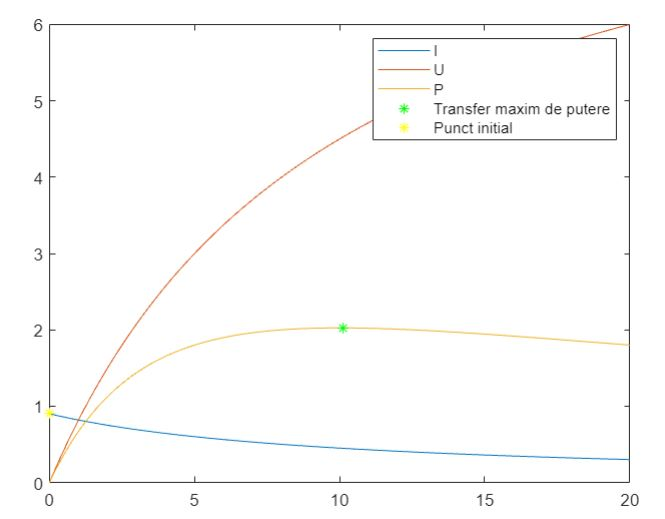
\includegraphics[scale=1]{grafic1.jpg}
\newpage
Funcția în matlab este:\\
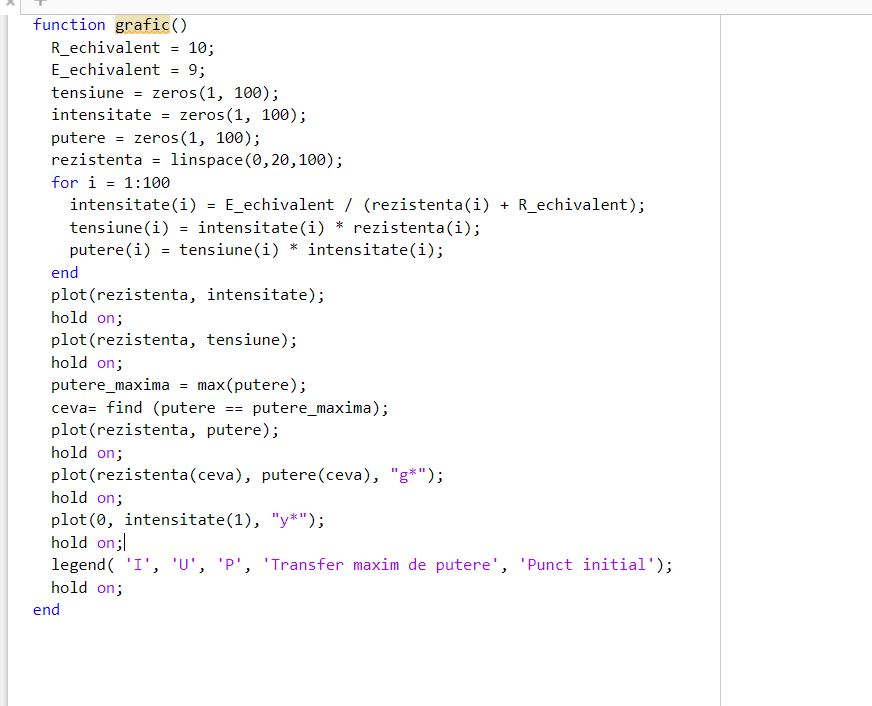
\includegraphics[scale=1]{grafic1.1.jpg}

\newpage
\section{Surse comandate, și simularea în Spice ale circuitelor cu surse comandate}
\subsection{SUCU}
Circuitul echivalent, cu o sursă de tensiune comandată în tensiune este:
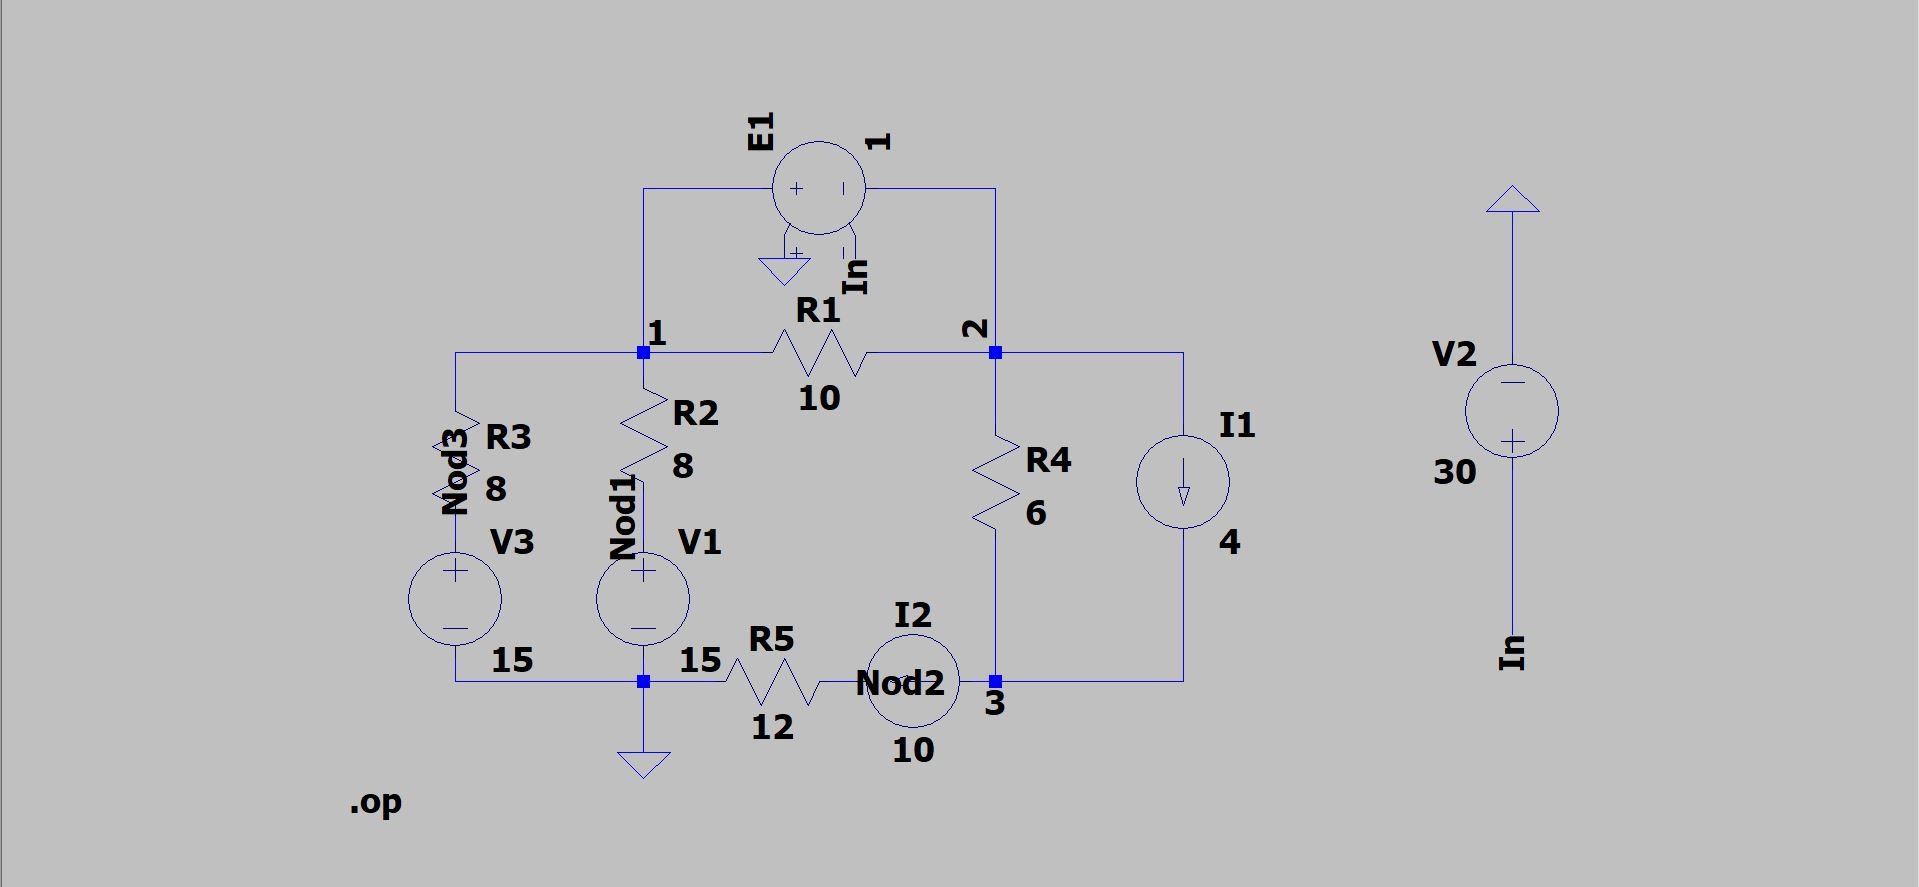
\includegraphics [scale=0.2]{sucu.jpg}

\subsection{Schema de rulare}
Schema de rulare, corespunzatoare circuitului din figura de mai sus este: 
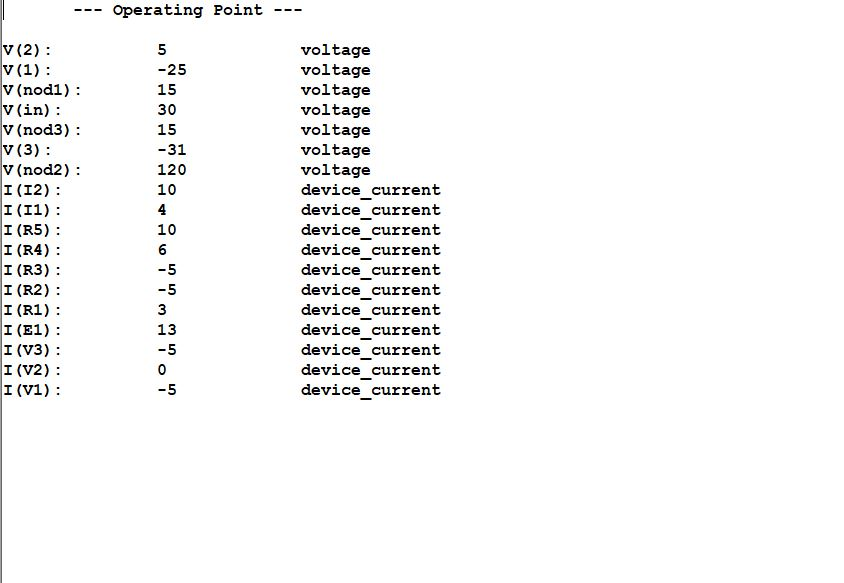
\includegraphics[width=10cm, height=10cm]{sucu-netlist.jpg}

\newpage
\section{Rezolvarea circuitelor de curent alternativ folosind instrumente software numerice}
Mai jos este prezentat circuitul sub forma sinusoidala:
\begin{center}
\begin{circuitikz}[american]
\draw (0, 2) to[R, l_=$R_3$,a^=8<\ohm>] (0, 4);
\draw (0,2) to[V>=21.2sin(100$\pi$)V] (0,0);
\draw (0,4) to[short] (4,4);
\draw (0,0) to[short] (4,0)node[label={[font=\footnotesize]below:$(4)$}] {};
\draw (4,6.5) to[short] (4,4)node[label={[yshift=0.2cm, xshift=-7]right:$(1)$}]{};\draw[blue] (4, 4) to[R, l_=$R_2$,a^=8<\ohm>, color=blue] (4, 2.5);
\draw[blue] (4, 2.5) to[V<=21.2sin(100$\pi$+$\frac{\pi}{4}$)V, color=blue] (4, 0);
\draw[blue] (4, 4) to[R, l_=$R_1$,a^=10<\ohm>, color=blue] (7, 4);
\draw (4, 0) to[R, l_=$R_5$,a^=12<\ohm>] (6.5, 0);
\draw (6.5,0) to[short] (7.5,0);
\draw (9, 0) to [I>=14.2sin(100$\pi$) A] (7.5,0) {};
\draw[blue] (9, 4) to[R, l_=$R_4$,a^=6<\ohm>, color=blue] (9, 0);
\draw[blue] (7,4) to [american inductor, a^=$\frac{1}{\pi}$H ,color=blue](9,4);
\draw (11,4) to[short] (9,4)node[label={[yshift=0.2cm, xshift=-7]right:$(2)$}]{};;
\draw (9,4) to[short] (9,6.5);
\draw (9,6.5) to[V<=42.2sin(100$\pi$)V] (4,6.5);
\draw (11, 0) to[short] (9,0)node[label={[yshift=0.2cm, xshift=-7]right:$(3)$}] {};
\draw (11, 4) to[I>=5.7sin(100$\pi$+$\frac{\pi}{4}$)A] (11, 2) node[label={[font=\footnotesize]}]{};
\draw (11,0) to [C, a^=$\frac{6}{10^{4}\pi}$F] ++(0,2);
\end{circuitikz}
\end{center}
\newpage
Circuitul sub forma algebrica este:
\begin{center}
\begin{circuitikz}[american]
\draw (0, 2) to[R, l_=$R_3$,a^=8<\ohm>] (0, 4);
\draw (0,2) to[V>=$\frac{15\sqrt{2}}{2}$(1+j)V] (0,0);
\draw (0,4) to[short] (4,4);
\draw (0,0) to[short] (4,0)node[label={[font=\footnotesize]below:$(4)$}] {};
\draw (4,6.5) to[short] (4,4)node[label={[yshift=0.2cm, xshift=-7]right:$(1)$}]{};\draw[blue] (4, 4) to[R, l_=$R_2$,a^=8<\ohm>, color=blue] (4, 2.5);
\draw[blue] (4, 2.5) to[V<=$\frac{15\sqrt{2}}{2}$(1+j)V, color=blue] (4, 0);
\draw[blue] (4, 4) to[R, l_=$R_1$,a^=10<\ohm>, color=blue] (7, 4);
\draw (4, 0) to[R, l_=$R_5$,a^=12<\ohm>] (6.5, 0);
\draw (6.5,0) to[short] (7.5,0);
\draw (9, 0) to [I>=10 A] (7.5,0) {};
\draw[blue] (9, 4) to[R, l_=$R_4$,a^=6<\ohm>, color=blue] (9, 0);
\draw[blue] (7,4) to [american inductor, a^=$10j$ ,color=blue](9,4);
\draw (11,4) to[short] (9,4)node[label={[yshift=0.2cm, xshift=-7]right:$(2)$}]{};;
\draw (9,4) to[short] (9,6.5);
\draw (9,6.5) to[V<=30V] (4,6.5);
\draw (11, 0) to[short] (9,0)node[label={[yshift=0.2cm, xshift=-7]right:$(3)$}] {};
\draw (11, 4) to[I>=$\frac{4\sqrt{2}}{2}$(1+j)A] (11, 2) node[label={[font=\footnotesize]}]{};
\draw (11,0) to [C, a^=$\frac{-100}{6}$j] ++(0,2);
\end{circuitikz}
\end{center}

Pentru cele 2 secțiuni alese, vom scrie teorema Kirchhoff I, și mai exact în nodurile
\{4\} și \{3\}.
\begin{equation}
\systeme{{1}:2*\frac{U_{41}+\frac{15\sqrt{2}}{2}(1+j)}{8}=10,
{2}:\frac{U{32}}{6}+10=\frac{4\sqrt{2}}{2}(1+j)}
\end{equation}
Efectuând calculele ajungem la rezultatele:$U_{41}=29,4-10,6j V$ și \\ $U_{32}=-43,03+17jV$ la fel cum se poate observa și-n graful de tensiunui, scris la început.\\
Scriptul pentru aflarea lui $U_{41}$ +$U_{32}$ este:\\
$U_{41}=\frac{40-15*\sqrt{2}*(1+j)}{2} $
\\
$U_{32}=(\frac{4*\sqrt(2)*(1+j)}{2}-10)*6$
\end{document}

